\documentclass[11pt,letterpaper]{article}
\usepackage[spanish]{babel}
%\usepackage[ansinew]{inputenc}
\usepackage[utf8]{inputenc}
%\usepackage[latin1]{inputenc}
\usepackage[letterpaper,includeheadfoot, top=0.5cm, bottom=3.0cm, right=2.0cm, left=2.0cm]{geometry}
\renewcommand{\familydefault}{\sfdefault}

\usepackage{graphicx}
\usepackage{color}
\usepackage{hyperref}
\usepackage{amssymb}
\usepackage{url}
%\usepackage{pdfpages}
\usepackage{fancyhdr}
\usepackage{hyperref}
\usepackage{subfig}

\usepackage{listings} %Codigo
\lstset{language=C, tabsize=4,framexleftmargin=5mm,breaklines=true}

\definecolor{gray}{rgb}{0.51,0.51,0.51}
\begin{document}
%\begin{sf}
% --------------- ---------PORTADA --------------------------------------------
\newpage
\pagestyle{fancy}
\fancyhf{}
%-------------------- CABECERA ---------------------
\fancyhead[L]{ 
\includegraphics[scale=0.9]{img/logo_die.pdf} }
%------------------ TÍTULO -----------------------
\vspace*{6cm}
\begin{center}
\Huge  {Estructura del Capítulo 3 del Informe de Memoria} \\
\vspace{1cm}
\huge {EL6908 - Introducción al Trabajo de Título}\\
\vspace{1cm}
\huge {\textit{Diseño e Implementación del Software de Control para el Computador a Bordo de un Pico-Satélite}}\\
%\vspace{1cm}
%\small {Título pequeño} 
\end{center}
%----------------- NOMBRES ------------------------
\vfill
\begin{flushright}
\begin{tabular}{ll}
\textbf{Autor} &: Carlos González C.\\
\textbf{Profesor Guía} &: Marcos Díaz Q.\\
\textbf{Profesor EL6908} &: Jorge Lopez H.\\
& \today\\
& Santiago, Chile.
\end{tabular}
\end{flushright}

% ·············· ENCABEZADO ············
\newpage
\pagestyle{fancy}
\fancyhf{}
%\fancyhead[L]{\rightmark}
\fancyhead[L]{\small \rm \textit{Sección \rightmark}}
\fancyhead[R]{\small \rm \textbf{\thepage}}
\fancyfoot[L]{\small \rm \textit{Estructura del capítulo 3}}
\fancyfoot[R]{\small \rm \textit{EL6908 - Introducción al Trabajo de Título}}
%\fancyfoot[C]{\thepage}
\renewcommand{\sectionmark}[1]{\markright{\thesection.\ #1}}
\renewcommand{\headrulewidth}{0.5pt}
\renewcommand{\footrulewidth}{0.5pt}

% =============== INDICE ===============

\tableofcontents
\listoffigures
\listoftables

% =============== ANALISIS ===============
\newpage
\section{Plan de trabajo}

El plan de trabajo para este proyecto detallado en la tabla \ref{plan_trabajo} se ha divido en etapas que contemplan ciertas tareas específicas a realizar para avanzar en el proyecto.

%···················· FIGURE ····················
\begin{table}[!ht]
\centering
\caption{Plan de trabajo} \label{plan_trabajo}
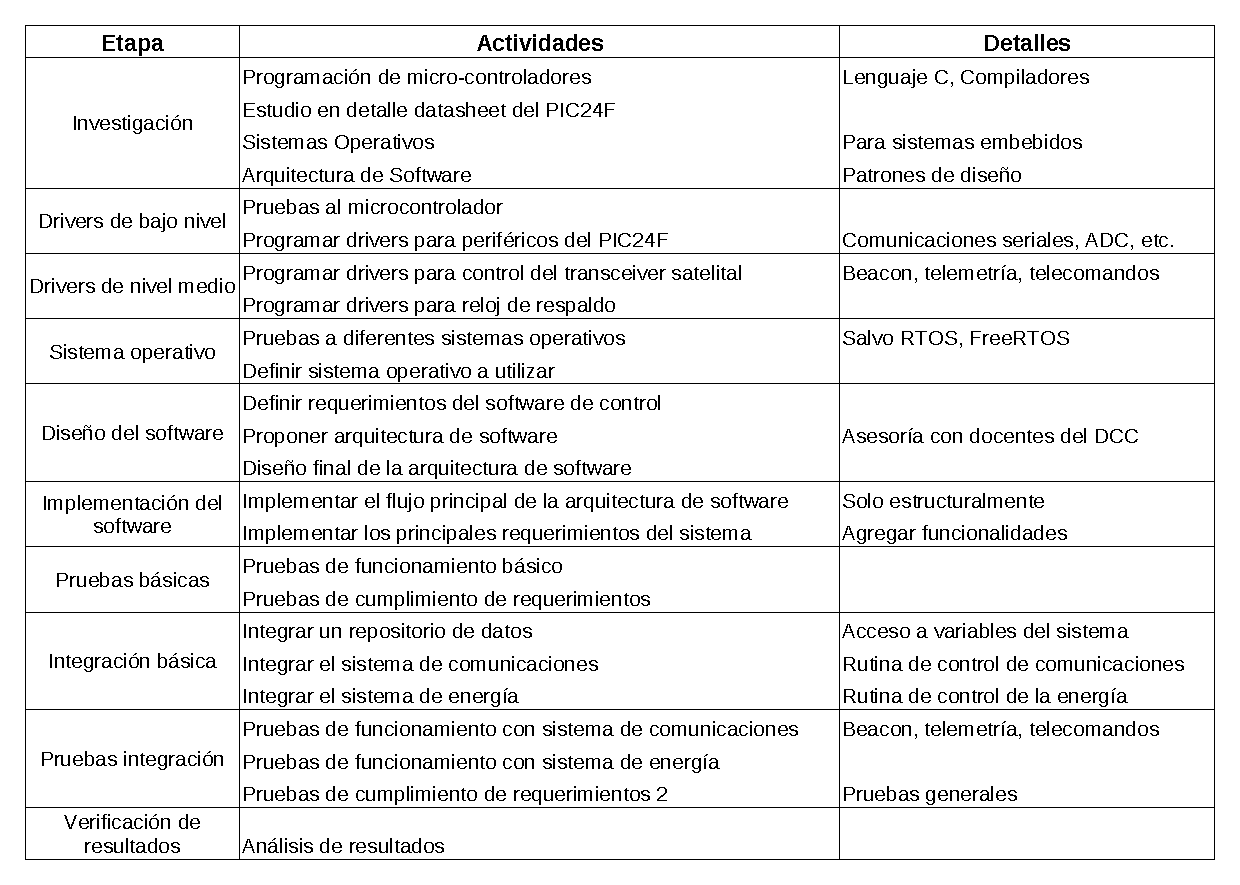
\includegraphics[width=\textwidth]{img/plan_trabajo.pdf}
\end{table}
%················································

\section{Carta Gantt}

El detalle del plan de trabajo se controla a través de la carta Gantt disponible en la tabla \ref{gantt} que considera las principales actividades e hitos que cumplir. Se consideran los tiempo de diseño e implementación del trabajo de memoria con sus dependencias de manera explícita así como también los tiempos asociados al desarrollo del informe del curso EL6908 y la redacción de la memoria en sí.

%···················· FIGURE ····················
\begin{figure}[!hb]
\centering
\caption{Carta Gantt} \label{gantt}
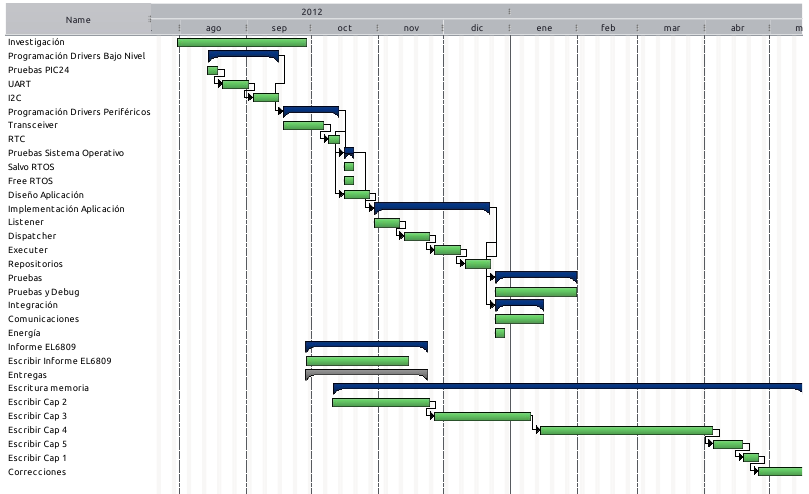
\includegraphics[width=\textwidth]{img/carta_gantt.png}
\end{figure}
%················································

% % ============= BIBLIOGRAFIA ==============
% \newpage
% \begin{thebibliography}{5}
% 	\bibitem{cmos} R. Jacob Baker, \textit{CMOS. Circuit Design, Layout, and Simulation}, 2nd ed., USA: IEEE Press, 2005
% 	
% \end{thebibliography}

\end{document}

% % ················ IMAGEN ·················
% \begin{figure}[ht!]
% \centering
% \fbox{\includegraphics[scale=0.6]{img/flujo.png}}
% \caption{Flujo de caja anual}\label{flujo}
% \end{figure}
% %··········································

% % ················ IMAGEN ·················
% \begin{figure}[ht!] \centering
% \subfloat[Esquemático]{\includegraphics[scale=0.44]{img/seguidor.png}}
% \subfloat[Simulación]{\includegraphics[scale=0.45]{img/seguidor1.png}}
% \caption{Simulación como seguidor de voltaje}\label{seguidor}
% \end{figure}
% %··········································